\section{Closing the compiler-feedback structural loop}
\label{sec:native-workflow-feedback}
\subsection{A fresh finite study, not a repaired stopped experiment}
The preceding stopped study and technical probes do not supply complete own
institutions or a final selection. We therefore conduct a separate prospective
campaign at source \code{7f1fc61f}, preserving the original scientist world,
two controls, T/U objectives, four-year horizon and reused development seed
61001. The local 35B designer proposes phases and connections among existing
typed ports; mechanism source, parameters and nodes are fixed in this slice.
This authoring interface is deliberately narrower than the general code-and-
graph framework, not evidence that broader freedom has been exercised here.

The campaign uses schema-formatted thinking output, a 57,344-token context,
16,384-output-token allowance and finite transport limits. Known invalid
proposals consume slots. The unchanged compiler's exact error, offending
causal-edge witnesses and original-input hashes can enter a later proposal's
history; no submitted graph is repaired. The actual history projection carries
these diagnostics from the original result boundary, rather than assuming a
recursive prior-request object. Six proposals are interleaved T0, U0, U1, T1,
T2, U2, with separate objective histories. Seven directed readiness calls and
six free proposals are recorded. Directed controls are not free-design evidence.

The original process normally closes after all six slots, with four complete
own worlds, two generation nulls and both complete controls. Two original-source
audits, cost exports and objective reports agree byte-for-byte, as do separate
choice, effect and full-model-input readouts. These are repeatable analyses
of one development history, not independent optimizer replications.

\begin{table}[t]
\centering\small
\begin{tabular}{llrrl}
\toprule
System/slot & Outcome & T & U & Literal own edit\\
\midrule
Original R7 & Complete & $-18$ & $-13.3333$ & Reference\\
Hand timing/routing & Complete & $-20$ & $-15.3333$ & Reference\\
T0 & Complete & $-20$ & $-15.3333$ & Three phase values\\
U0 & Complete & $-20$ & $-15.3333$ & Explicit parent retention\\
U1 & Generation null & --- & --- & Invalid causal order\\
T1 & Complete & $-20$ & $-15.3333$ & Explicit parent retention\\
T2 & Generation null & --- & --- & Required inputs removed\\
U2 & Complete & $-20$ & $-15.3333$ & One phase value\\
\bottomrule
\end{tabular}
\caption{Every control and consumed proposal in the normally closed
compiler-feedback study. Both losses are evaluated on each complete physical
world. Nulls have no scientific loss. Display rounding is not used for
selection. T0/T1 tie under T; U0/U2 tie under U; chronological first-tie
selection retains T0 and U0. All complete own outputs tie the hand control.}
\label{tab:workflow-feedback-all-slots}
\end{table}

\begin{figure}[t]
\centering
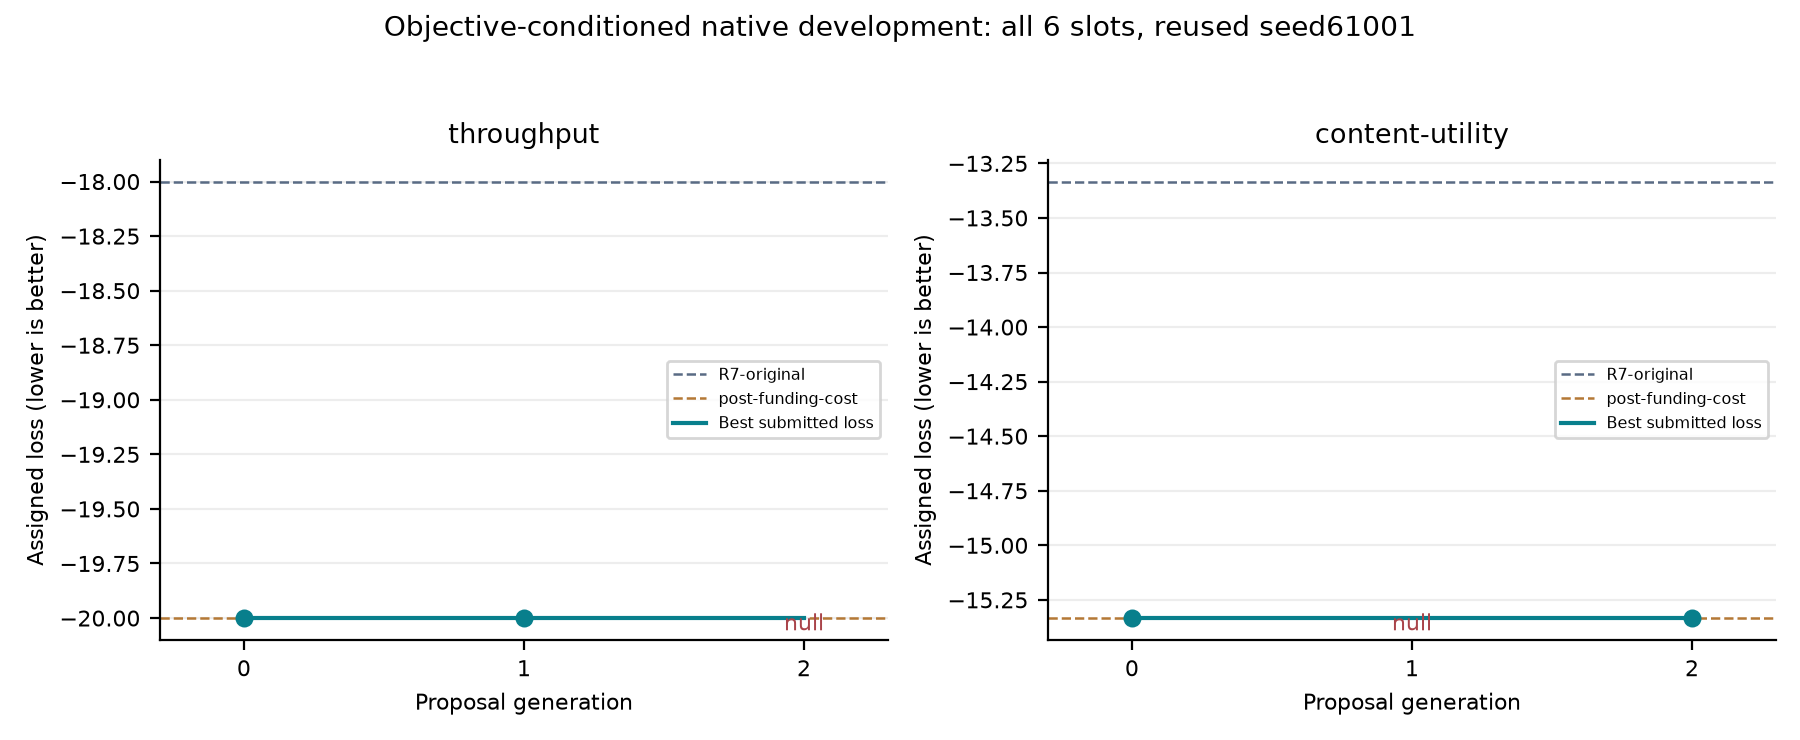
\includegraphics[width=\linewidth]{figures/native-workflow-compiler-feedback-v2/objective-loss-paths.png}
\caption{The complete objective-conditioned development paths. Dashed lines
show both references; markers show complete own evaluations and the solid
line their best submitted loss. Invalid proposals remain labeled null, not
assigned a penalty or replaced. No own gain over the hand incumbent occurs.
This is one reused development seed, without independent error bars.}
\label{fig:workflow-feedback-paths}
\end{figure}

\subsection{Phase labels are not necessarily behavioral changes}
T0 changes the director, effect consumer and cost phases from 161/162/163 to
163/164/165, but leaves connections and the actual total annual order
unchanged. U2 changes only the cost phase from 163 to 165. U0 and T1 explicitly
retain their parent. All four complete own systems and the hand control issue
the same ordered 127 full scientist request payloads and receive the same
literal response choices, including recorded finish metadata. Provider
envelopes differ and remain unmodified. R7 instead has 115 requests and forms
the second observed input class. Thus six physical completions yield only two
observed full-input classes, not six behaviorally independent institutions.
Equality on these histories is not global program equivalence or permission
to skip future worlds.

The two invalid proposals are also informative about the actual search path.
U1 places cost collection at 175 while retaining its outgoing zero-latency
edge to communication at 170. T2 removes required selection inputs and puts
consumers before connected producers. These are known final replies, not
unknown transport completions. The actual U2 request contains U1's exact
failure witness. U2 then compiles, but this uncontrolled sequence does not
identify a feedback benefit. Some designer rationales assert parent violations
or optimality unsupported by the received graph and loss definition; those
assertions are not host-implemented rules or proofs of effectiveness.

Across this campaign there are 750 complete scientist responses, 75 physical
content-critic calls and no scientist wire without a committed reply. Recorded
scientist usage totals 937,108 prompt and 77,254 completion tokens. Free-design
calls use 147,740 input and 46,206 output tokens including thinking; readiness
uses another 169,711 and 5,490. Science wall time is 6,082.936 seconds on shared
local hardware. Token accounting and wall time do not establish GPU FLOPs,
energy, monetary cost or dedicated-device throughput.

\subsection{What this closure establishes, and what remains}
This campaign establishes an operated proposal--failure-feedback--native-
evaluation--selection loop, not an automatically invented improvement. Its
chosen parent is already the hand timing/routing control. Retaining that
parent, or changing inert phase labels, cannot be presented as discovering
the control's advantage over R7. No successful own wiring change occurs.

There is also a concrete headroom question before simply adding repetitions.
At the inspected original initialization, each of five researchers has a
shortest expertise duration of two years. Under serial uninterrupted catalog
projects, two outputs per project, no extra producers or authors, and at most
one acceptance occurrence per output, the conditional four-year envelope is
$2\sum_{i=1}^{5}\lfloor4/2\rfloor=20$. The hand reaches this conditional
value. This is not a theorem over all allowed graphs, resubmission paths,
decision occurrences or other initializations. U also depends on content, so
neither its optimum nor a necessary T/U trade-off follows from the count.

Before seeing own outcomes, a separate note fixed one hash-derived evaluation
seed, 1858637637. Selection-fixed evaluation must preserve both own labels and
both controls regardless of development improvement; literal identity alone
may share physical jobs. Its initial preparation stops before inference when
the usage inventory encounters non-production unit-test stores. That failed
preparation supplies no evaluation scores. A separately declared explicit-
fixture inventory correction passes focused tests and a nine-world scripted
native handoff with double cold audits; that is software evidence, not a
completed held-out comparison. One unused seed would in any event not establish stable advantage
or independent optimizer histories. Broader code/mechanism freedom and an
important independently supported objective-to-system result remain open.
\FloatBarrier
